%=======================02-713 LaTeX template, following the 15-210 template==================
%
% You don't need to use LaTeX or this template, but you must turn your homework in as
% a typeset PDF somehow.
%
% How to use:
%    1. Update your information in section "A" below
%    2. Write your answers in section "B" below. Precede answers for all 
%       parts of a question with the command "\question{n}{desc}" where n is
%       the question number and "desc" is a short, one-line description of 
%       the problem. There is no need to restate the problem.
%    3. If a question has multiple parts, precede the answer to part x with the
%       command "\part{x}".
%    4. If a problem asks you to design an algorithm, use the commands
%       \algorithm, \correctness, \runtime to precede your discussion of the 
%       description of the algorithm, its correctness, and its running time, respectively.
%    5. You can include graphics by using the command \includegraphics{FILENAME}
%
\documentclass[11pt]{article}
\usepackage{amsmath,amssymb,amsthm}
\usepackage{tikz}
\usetikzlibrary{arrows,positioning, calc}
\tikzstyle{vertex}=[draw,fill=black!15,circle,minimum size=20pt,inner sep=0pt]
\usepackage{graphicx}
\usepackage[margin=1in]{geometry}
\usepackage{fancyhdr}
\usepackage{mathtools}
\usepackage{placeins}
\usepackage{listings}
\usepackage{color}
\usepackage{forest}
\usepackage{tikz}
\usepackage{caption}
\usepackage{mathtools}
\DeclarePairedDelimiter{\ceil}{\lceil}{\rceil}
\DeclarePairedDelimiter{\floor}{\lfloor}{\rfloor}

\definecolor{dkgreen}{rgb}{0,0.6,0}
\definecolor{gray}{rgb}{0.5,0.5,0.5}
\definecolor{mauve}{rgb}{0.58,0,0.82}

\lstset{frame=none,
  language=Java,
  aboveskip=3mm,
  belowskip=3mm,
  showstringspaces=false,
  columns=flexible,
  basicstyle={\small\ttfamily},
  numbers=none,
  numberstyle=\tiny\color{gray},
  keywordstyle=\color{blue},
  commentstyle=\color{dkgreen},
  stringstyle=\color{mauve},
  breaklines=true,
  breakatwhitespace=true,
  tabsize=3
}

\setlength{\parindent}{0pt}
\setlength{\parskip}{5pt plus 1pt}
\setlength{\headheight}{13.6pt}
\newcommand\question[2]{\vspace{.25in}\hrule\textbf{#1 #2}\vspace{.5em}\hrule\vspace{.10in}}
\renewcommand\part[1]{\vspace{.10in}\textbf{(#1)}}
\newcommand\algorithm{\vspace{.10in}\textbf{Algorithm: }}
\newcommand\correctness{\vspace{.10in}\textbf{Correctness: }}
\newcommand\runtime{\vspace{.10in}\textbf{Running time: }}
\pagestyle{fancyplain}
\lhead{\textbf{\NAME}}
\chead{\textbf{HW\HWNUM}}
\rhead{\today}
\begin{document}\raggedright
%Section A==============Change the values below to match your information==================
\newcommand\NAME{Sean Connor (443-414-5111)}  % your name
\newcommand\HWNUM{4}              % the homework number
%Section B==============Put your answers to the questions below here=======================
\question{Q1}{   CLRS 6.2-1}
\part{a}
Here follows an illustration of Max-Heapify(A,3) on $A<27,17,3,16,13,10,1,5,7,12,4,6,9,0>$.

\begin{figure}[htbp!]
\centering
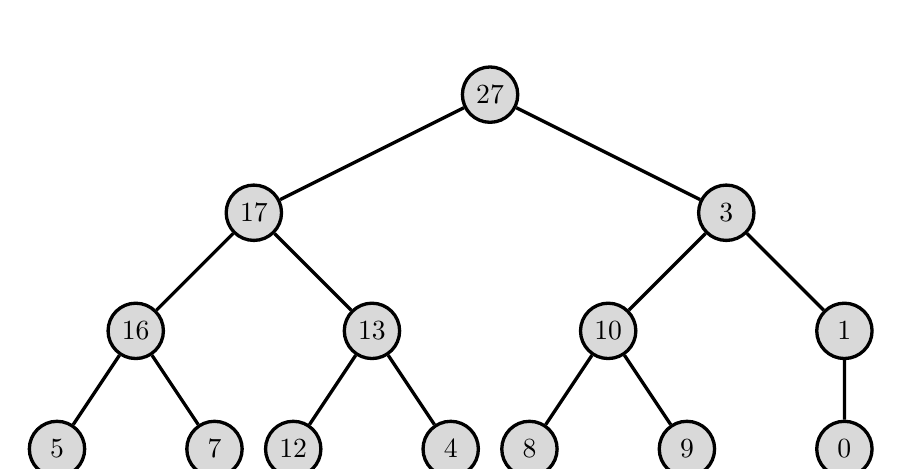
\begin{tikzpicture}[very thick,level/.style={sibling distance=60mm/#1}]
\node [vertex] {$27$}
  child {node [vertex] {$17$}
    child {node [vertex] {$16$}
      child {node [vertex] {$5$}}
      child {node [vertex] {$7$}}
    }
    child {node [vertex] {$13$}
      child {node [vertex] {$12$}}
      child {node [vertex] {$4$}}
    }
  }
  child {node [vertex] {$3$}
    child {node [vertex] {$10$}
      child {node [vertex] {$8$}}
      child {node [vertex] {$9$}}
    }
    child {node [vertex] {$1$}
      child {node [vertex] {$0$}}
    }
  };
\end{tikzpicture}
\end{figure}

\begin{figure}[htbp!]
\centering
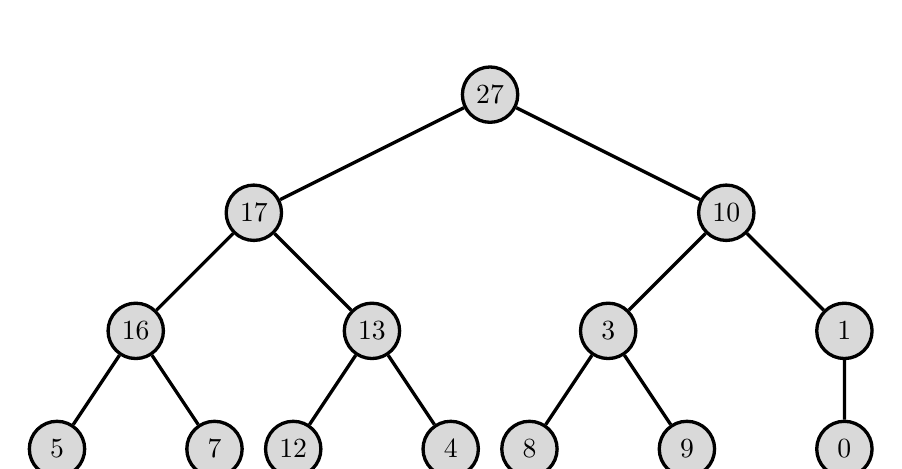
\begin{tikzpicture}[very thick,level/.style={sibling distance=60mm/#1}]
\node [vertex] {$27$}
  child {node [vertex] {$17$}
    child {node [vertex] {$16$}
      child {node [vertex] {$5$}}
      child {node [vertex] {$7$}}
    }
    child {node [vertex] {$13$}
      child {node [vertex] {$12$}}
      child {node [vertex] {$4$}}
    }
  }
  child {node [vertex] {$10$}
    child {node [vertex] {$3$}
      child {node [vertex] {$8$}}
      child {node [vertex] {$9$}}
    }
    child {node [vertex] {$1$}
      child {node [vertex] {$0$}}
    }
  };
\end{tikzpicture}
\end{figure}

\begin{figure}[htbp!]
\centering
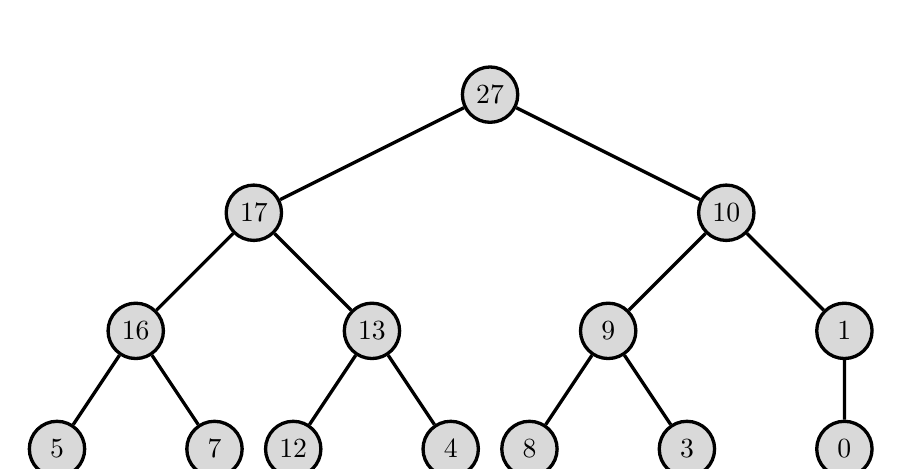
\begin{tikzpicture}[very thick,level/.style={sibling distance=60mm/#1}]
\node [vertex] {$27$}
  child {node [vertex] {$17$}
    child {node [vertex] {$16$}
      child {node [vertex] {$5$}}
      child {node [vertex] {$7$}}
    }
    child {node [vertex] {$13$}
      child {node [vertex] {$12$}}
      child {node [vertex] {$4$}}
    }
  }
  child {node [vertex] {$10$}
    child {node [vertex] {$9$}
      child {node [vertex] {$8$}}
      child {node [vertex] {$3$}}
    }
    child {node [vertex] {$1$}
      child {node [vertex] {$0$}}
    }
  };
\end{tikzpicture}
\end{figure}
\newpage


\part{b}
Here follows an illustration of Build-Max-Heap(A) on $A<5,3,17,10,84,19,6,22,4>$.

\begin{figure}[htbp!]
\centering
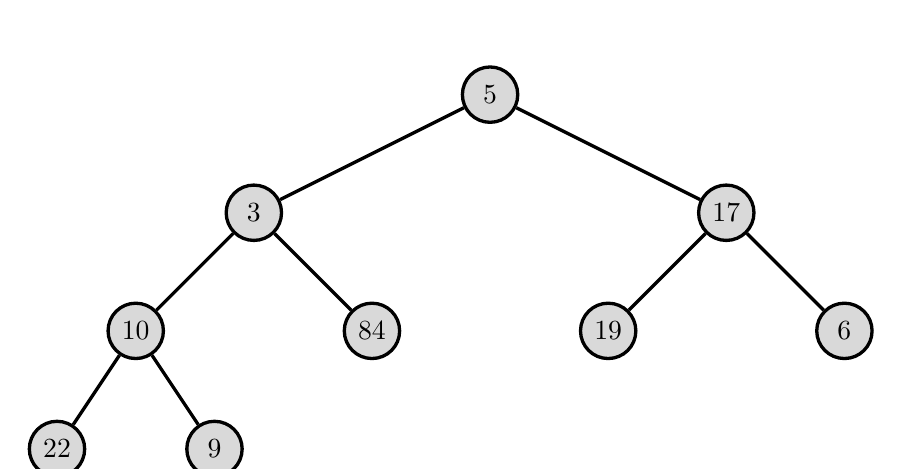
\begin{tikzpicture}[very thick,level/.style={sibling distance=60mm/#1}]
\node [vertex] {$5$}
  child {node [vertex] {$3$}
    child {node [vertex] {$10$}
      child {node [vertex] {$22$}}
      child {node [vertex] {$9$}}
    }
    child {node [vertex] {$84$}
    }
  }
  child {node [vertex] {$17$}
    child {node [vertex] {$19$}
    }
    child {node [vertex] {$6$}
    }
  };
\end{tikzpicture}
\end{figure}

\begin{figure}[htbp!]
\centering
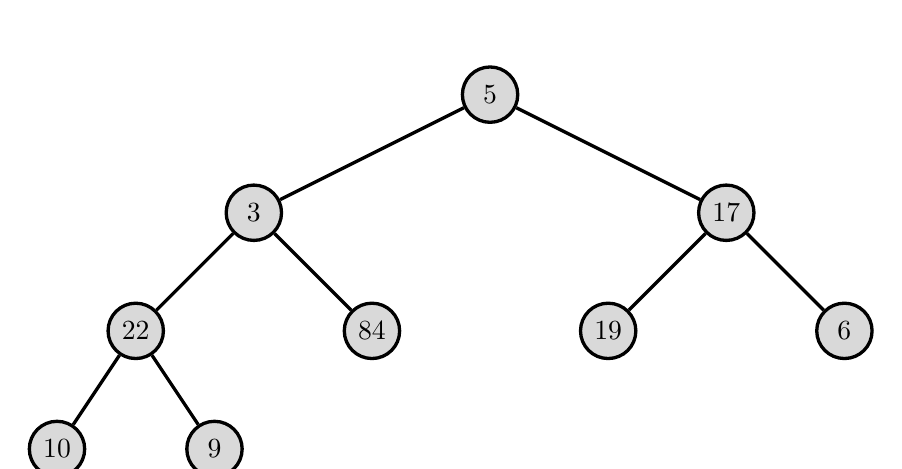
\begin{tikzpicture}[very thick,level/.style={sibling distance=60mm/#1}]
\node [vertex] {$5$}
  child {node [vertex] {$3$}
    child {node [vertex] {$22$}
      child {node [vertex] {$10$}}
      child {node [vertex] {$9$}}
    }
    child {node [vertex] {$84$}
    }
  }
  child {node [vertex] {$17$}
    child {node [vertex] {$19$}
    }
    child {node [vertex] {$6$}
    }
  };
\end{tikzpicture}
\end{figure}

\begin{figure}[htbp!]
\centering
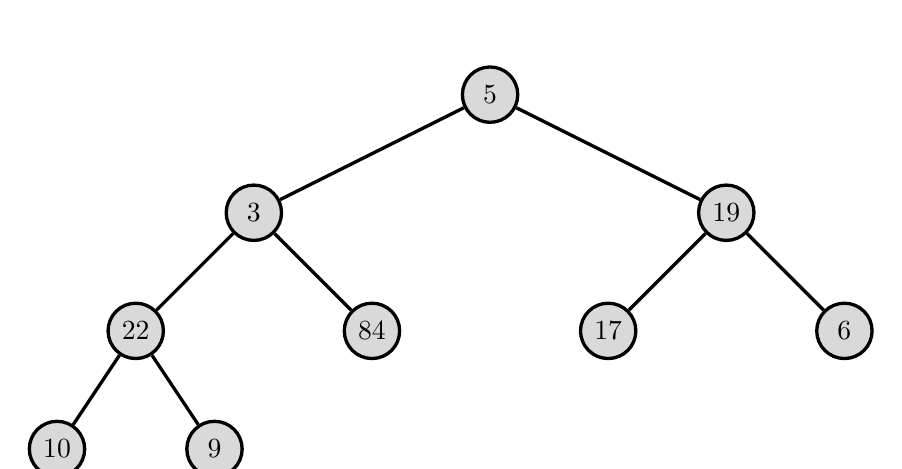
\begin{tikzpicture}[very thick,level/.style={sibling distance=60mm/#1}]
\node [vertex] {$5$}
  child {node [vertex] {$3$}
    child {node [vertex] {$22$}
      child {node [vertex] {$10$}}
      child {node [vertex] {$9$}}
    }
    child {node [vertex] {$84$}
    }
  }
  child {node [vertex] {$19$}
    child {node [vertex] {$17$}
    }
    child {node [vertex] {$6$}
    }
  };
\end{tikzpicture}
\end{figure}

\begin{figure}[htbp!]
\centering
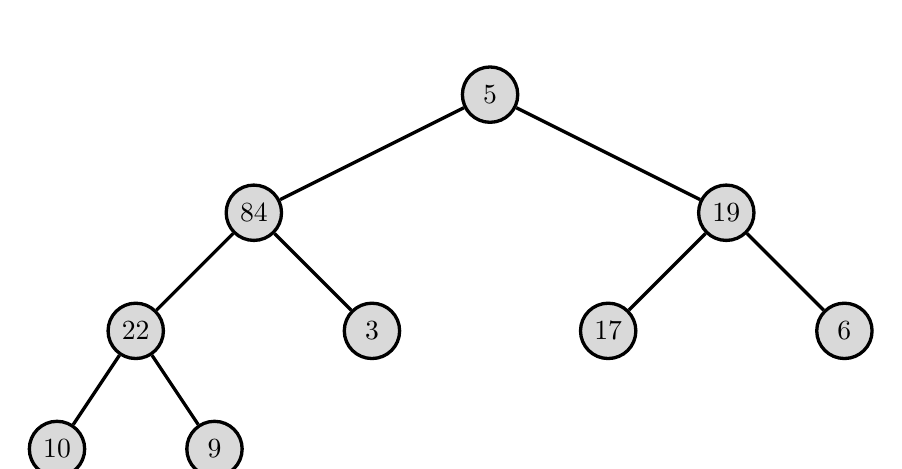
\begin{tikzpicture}[very thick,level/.style={sibling distance=60mm/#1}]
\node [vertex] {$5$}
  child {node [vertex] {$84$}
    child {node [vertex] {$22$}
      child {node [vertex] {$10$}}
      child {node [vertex] {$9$}}
    }
    child {node [vertex] {$3$}
    }
  }
  child {node [vertex] {$19$}
    child {node [vertex] {$17$}
    }
    child {node [vertex] {$6$}
    }
  };
\end{tikzpicture}
\end{figure}

\begin{figure}[htbp!]
\centering
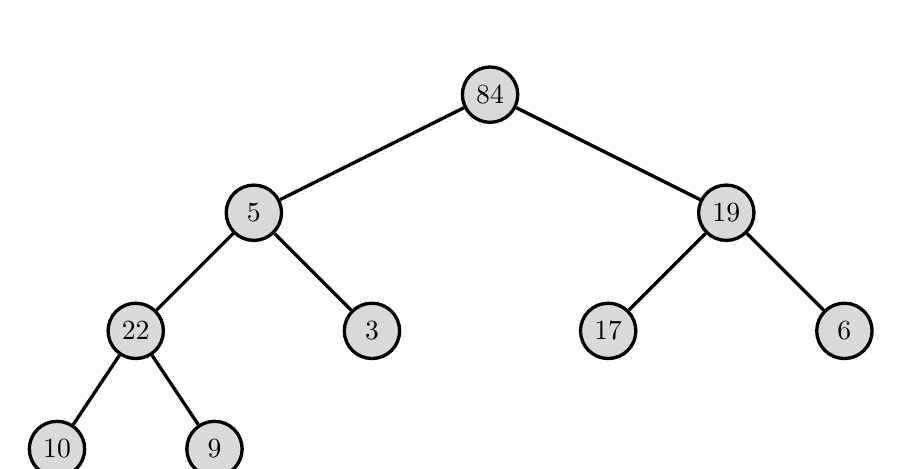
\begin{tikzpicture}[very thick,level/.style={sibling distance=60mm/#1}]
\node [vertex] {$84$}
  child {node [vertex] {$5$}
    child {node [vertex] {$22$}
      child {node [vertex] {$10$}}
      child {node [vertex] {$9$}}
    }
    child {node [vertex] {$3$}
    }
  }
  child {node [vertex] {$19$}
    child {node [vertex] {$17$}
    }
    child {node [vertex] {$6$}
    }
  };
\end{tikzpicture}
\end{figure}

\begin{figure}[htbp!]
\centering
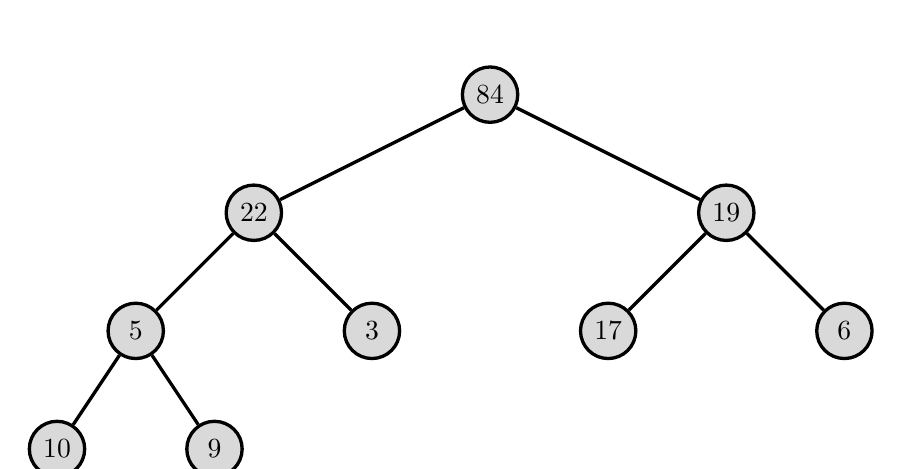
\begin{tikzpicture}[very thick,level/.style={sibling distance=60mm/#1}]
\node [vertex] {$84$}
  child {node [vertex] {$22$}
    child {node [vertex] {$5$}
      child {node [vertex] {$10$}}
      child {node [vertex] {$9$}}
    }
    child {node [vertex] {$3$}
    }
  }
  child {node [vertex] {$19$}
    child {node [vertex] {$17$}
    }
    child {node [vertex] {$6$}
    }
  };
\end{tikzpicture}
\end{figure}

\begin{figure}[htbp!]
\centering
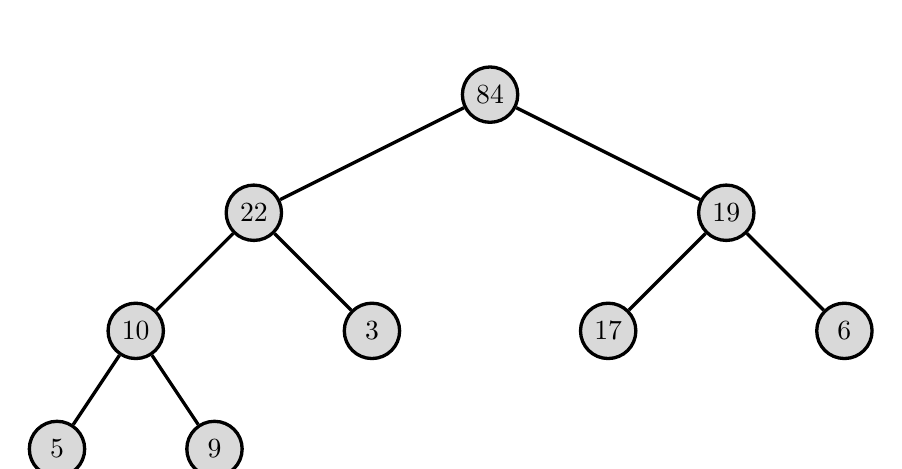
\begin{tikzpicture}[very thick,level/.style={sibling distance=60mm/#1}]
\node [vertex] {$84$}
  child {node [vertex] {$22$}
    child {node [vertex] {$10$}
      child {node [vertex] {$5$}}
      child {node [vertex] {$9$}}
    }
    child {node [vertex] {$3$}
    }
  }
  child {node [vertex] {$19$}
    child {node [vertex] {$17$}
    }
    child {node [vertex] {$6$}
    }
  };
\end{tikzpicture}
\end{figure}
\newpage

\part{c}
Here follows an illustration of Heapsort(A) on $A<5,13,2,25,7,17,20,8,4>$.

\begin{figure}[htbp!]
\centering
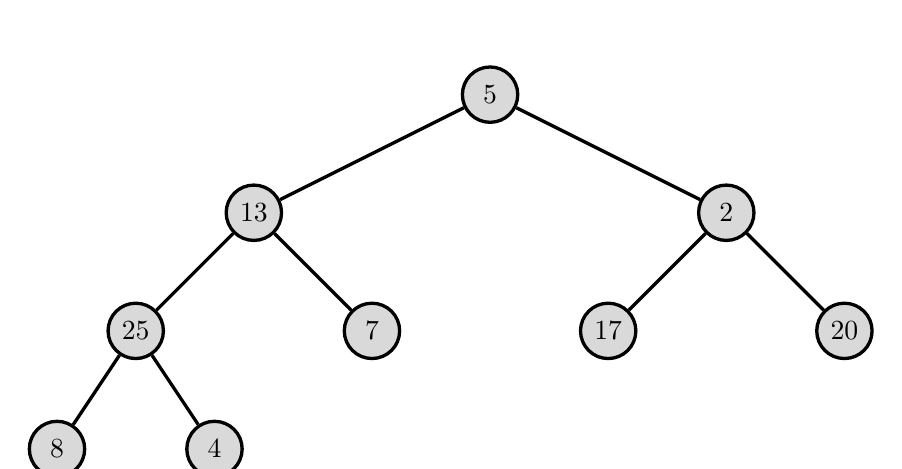
\begin{tikzpicture}[very thick,level/.style={sibling distance=60mm/#1}]
\node [vertex] {$5$}
  child {node [vertex] {$13$}
    child {node [vertex] {$25$}
      child {node [vertex] {$8$}}
      child {node [vertex] {$4$}}
    }
    child {node [vertex] {$7$}
    }
  }
  child {node [vertex] {$2$}
    child {node [vertex] {$17$}
    }
    child {node [vertex] {$20$}
    }
  };
\end{tikzpicture}
\caption*{}
\end{figure}

\begin{figure}[htbp!]
\centering
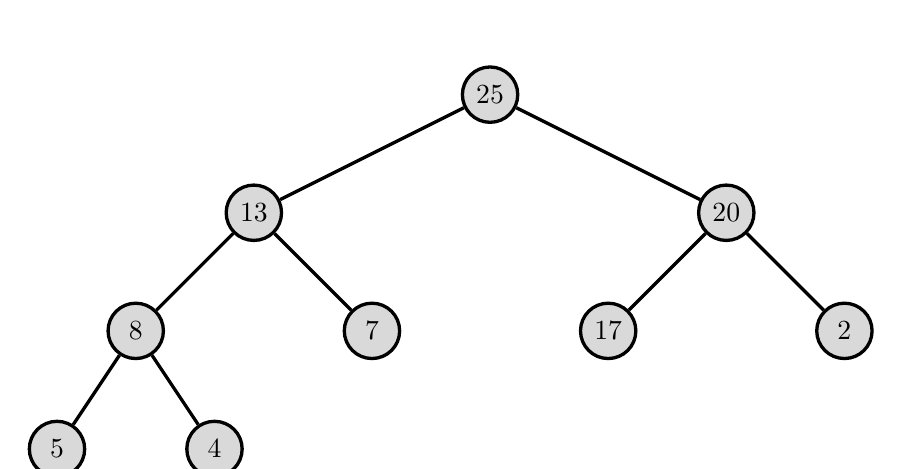
\begin{tikzpicture}[very thick,level/.style={sibling distance=60mm/#1}]
\node [vertex] {$25$}
  child {node [vertex] {$13$}
    child {node [vertex] {$8$}
      child {node [vertex] {$5$}}
      child {node [vertex] {$4$}}
    }
    child {node [vertex] {$7$}
    }
  }
  child {node [vertex] {$20$}
    child {node [vertex] {$17$}
    }
    child {node [vertex] {$2$}
    }
  };
\end{tikzpicture}
\caption*{Build-Max-Heap on A.}
\end{figure}

\begin{figure}[htbp!]
\centering
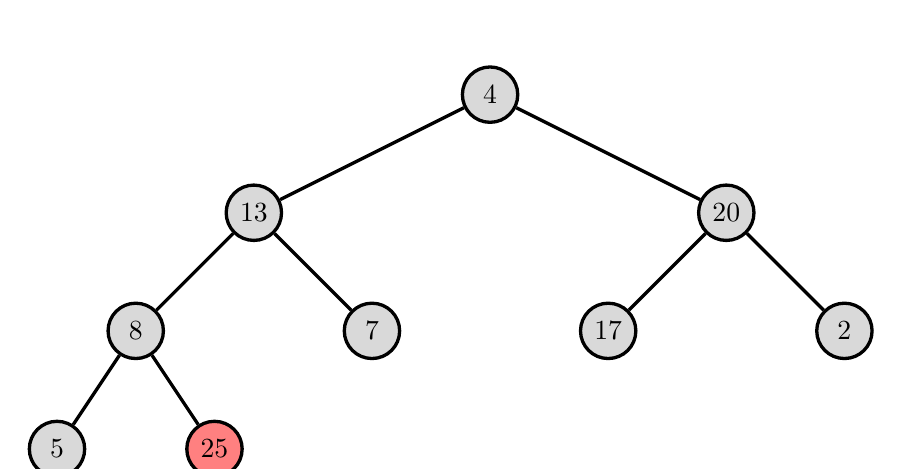
\begin{tikzpicture}[very thick,level/.style={sibling distance=60mm/#1}]
\node [vertex] {$4$}
  child {node [vertex] {$13$}
    child {node [vertex] {$8$}
      child {node [vertex] {$5$}}
      child {node [vertex, fill=red!50] {$25$}}
    }
    child {node [vertex] {$7$}
    }
  }
  child {node [vertex] {$20$}
    child {node [vertex] {$17$}
    }
    child {node [vertex] {$2$}
    }
  };
\end{tikzpicture}
\caption*{for i=A.length $\rightarrow$ 2 exchange A[1] with A[i], decrement heapsize, and Max-Heapify(A,1).}
\end{figure}

\begin{figure}[htbp!]
\centering
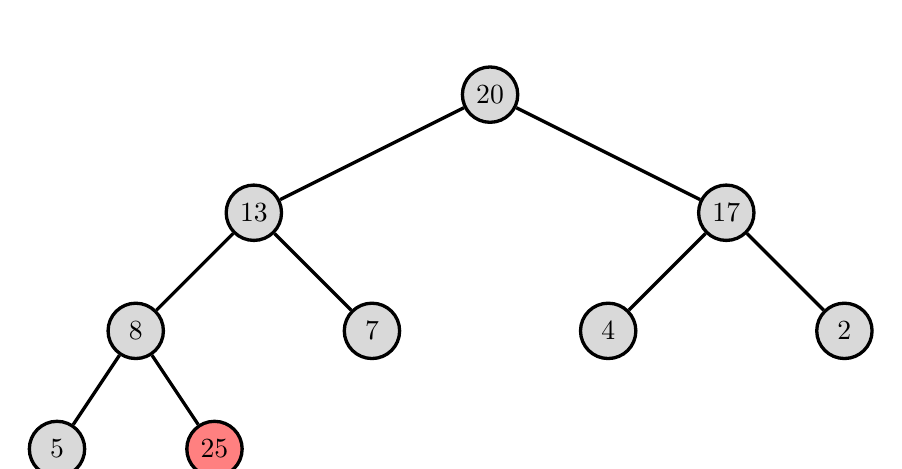
\begin{tikzpicture}[very thick,level/.style={sibling distance=60mm/#1}]
\node [vertex] {$20$}
  child {node [vertex] {$13$}
    child {node [vertex] {$8$}
      child {node [vertex] {$5$}}
      child {node [vertex, fill=red!50] {$25$}}
    }
    child {node [vertex] {$7$}
    }
  }
  child {node [vertex] {$17$}
    child {node [vertex] {$4$}
    }
    child {node [vertex] {$2$}
    }
  };
\end{tikzpicture}
\caption*{Reestablish heap.}
\end{figure}

\begin{figure}[htbp!]
\centering
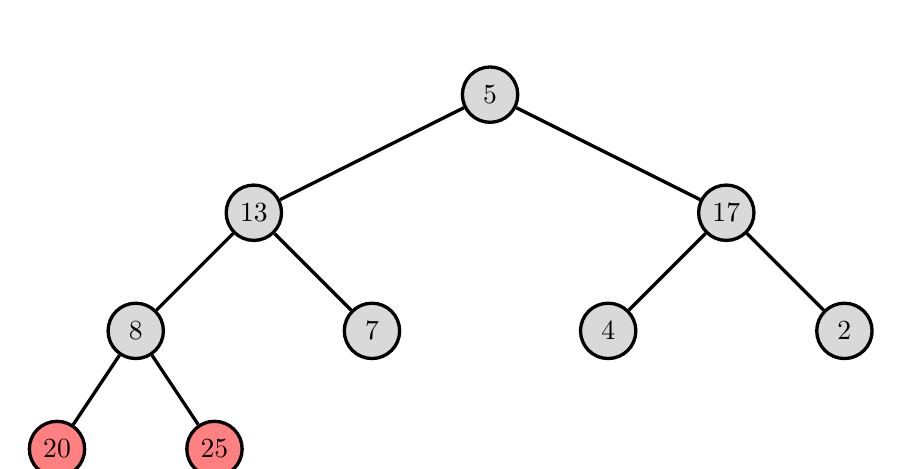
\begin{tikzpicture}[very thick,level/.style={sibling distance=60mm/#1}]
\node [vertex] {$5$}
  child {node [vertex] {$13$}
    child {node [vertex] {$8$}
      child {node [vertex, fill=red!50] {$20$}}
      child {node [vertex, fill=red!50] {$25$}}
    }
    child {node [vertex] {$7$}
    }
  }
  child {node [vertex] {$17$}
    child {node [vertex] {$4$}
    }
    child {node [vertex] {$2$}
    }
  };
\end{tikzpicture}
\caption*{Repeat...}
\end{figure}

\begin{figure}[htbp!]
\centering
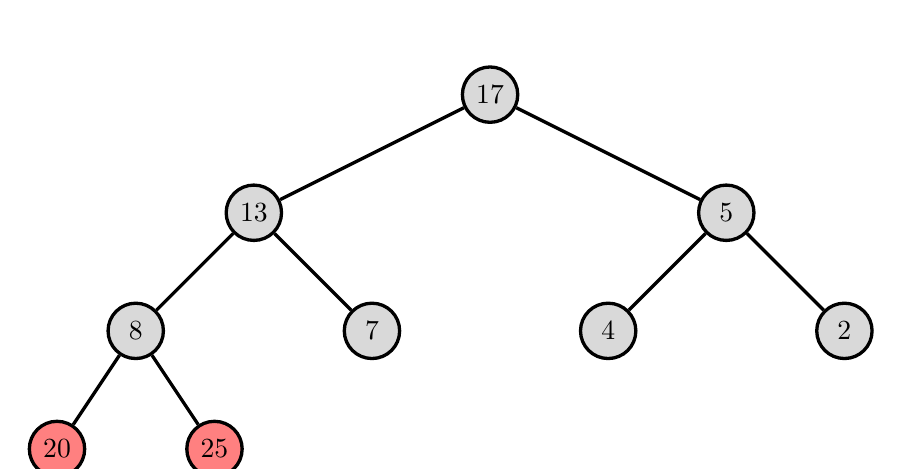
\begin{tikzpicture}[very thick,level/.style={sibling distance=60mm/#1}]
\node [vertex] {$17$}
  child {node [vertex] {$13$}
    child {node [vertex] {$8$}
      child {node [vertex, fill=red!50] {$20$}}
      child {node [vertex, fill=red!50] {$25$}}
    }
    child {node [vertex] {$7$}
    }
  }
  child {node [vertex] {$5$}
    child {node [vertex] {$4$}
    }
    child {node [vertex] {$2$}
    }
  };
\end{tikzpicture}
\caption*{Reestablish heap.}
\end{figure}

\begin{figure}[htbp!]
\centering
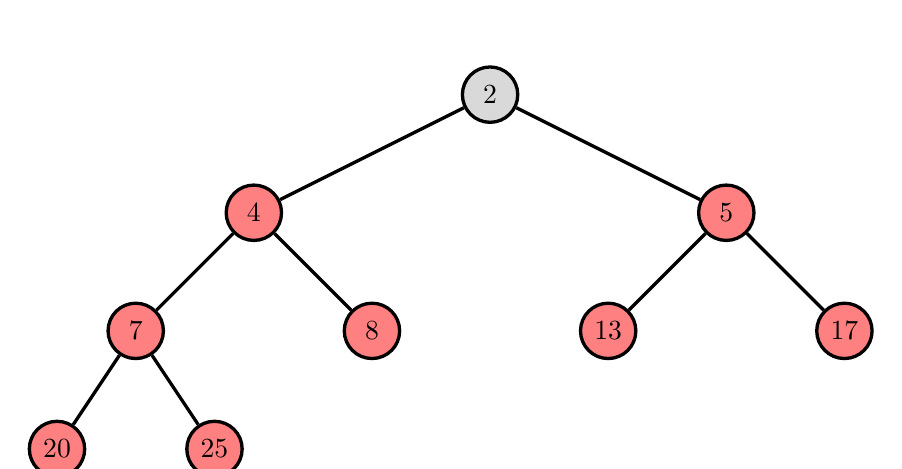
\begin{tikzpicture}[very thick,level/.style={sibling distance=60mm/#1}]
\node [vertex] {$2$}
  child {node [vertex, fill=red!50] {$4$}
    child {node [vertex, fill=red!50] {$7$}
      child {node [vertex, fill=red!50] {$20$}}
      child {node [vertex, fill=red!50] {$25$}}
    }
    child {node [vertex, fill=red!50] {$8$}
    }
  }
  child {node [vertex, fill=red!50] {$5$}
    child {node [vertex, fill=red!50] {$13$}
    }
    child {node [vertex, fill=red!50] {$17$}
    }
  };
\end{tikzpicture}
\caption*{Repeat until sorted (completion of for-loop).}
\end{figure}
\newpage

\part{d}
Here follows an illustration of Heap-Extract-Max(A) on $A<15,13,9,5,12,8,7,4,0,6,2,1>$.

\begin{figure}[htbp!]
\centering
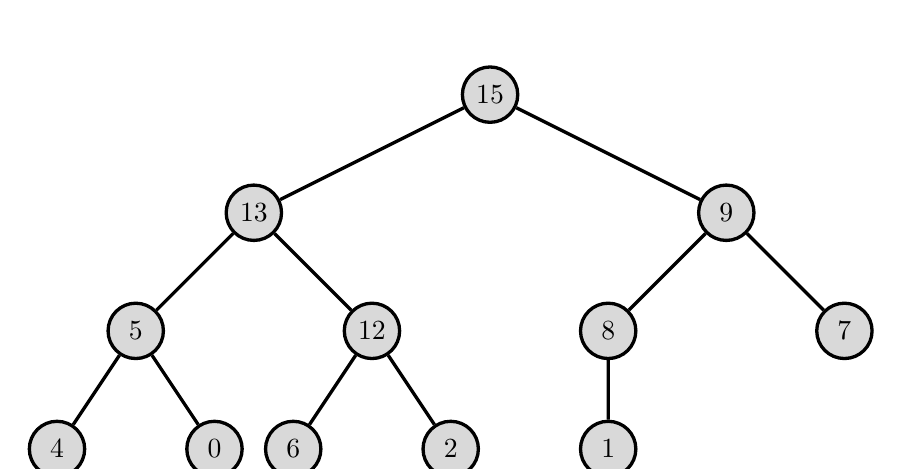
\begin{tikzpicture}[very thick,level/.style={sibling distance=60mm/#1}]
\node [vertex] {$15$}
  child {node [vertex] {$13$}
    child {node [vertex] {$5$}
      child {node [vertex] {$4$}}
      child {node [vertex] {$0$}}
    }
    child {node [vertex] {$12$}
      child {node [vertex] {$6$}}
      child {node [vertex] {$2$}}
    }
  }
  child {node [vertex] {$9$}
    child {node [vertex] {$8$}
      child {node [vertex] {$1$}}
    }
    child {node [vertex] {$7$}
    }
  };
\end{tikzpicture}
\caption*{}
\end{figure}

\begin{figure}[htbp!]
\centering
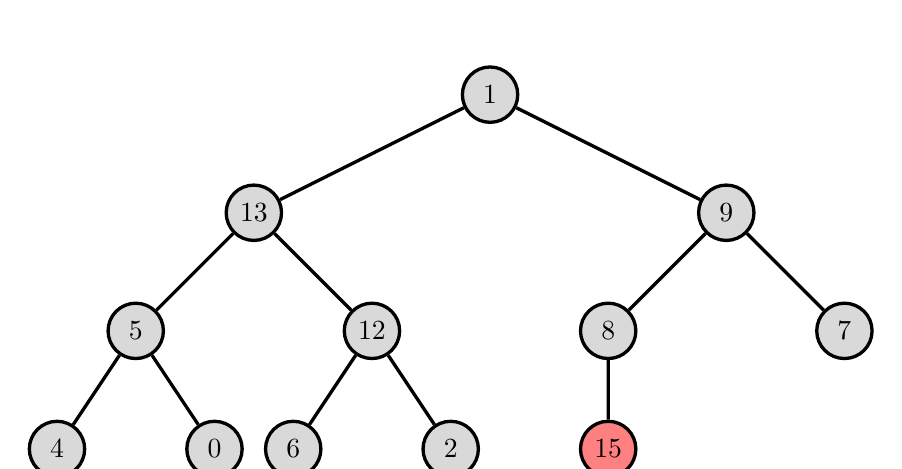
\begin{tikzpicture}[very thick,level/.style={sibling distance=60mm/#1}]
\node [vertex] {$1$}
  child {node [vertex] {$13$}
    child {node [vertex] {$5$}
      child {node [vertex] {$4$}}
      child {node [vertex] {$0$}}
    }
    child {node [vertex] {$12$}
      child {node [vertex] {$6$}}
      child {node [vertex] {$2$}}
    }
  }
  child {node [vertex] {$9$}
    child {node [vertex] {$8$}
      child {node [vertex, fill=red!50] {$15$}}
    }
    child {node [vertex] {$7$}
    }
  };
\end{tikzpicture}
\caption*{max = A[1] = 15 \\ A[1] = A[A.heapsize] = A[12] = 1}
\end{figure}

\begin{figure}[htbp!]
\centering
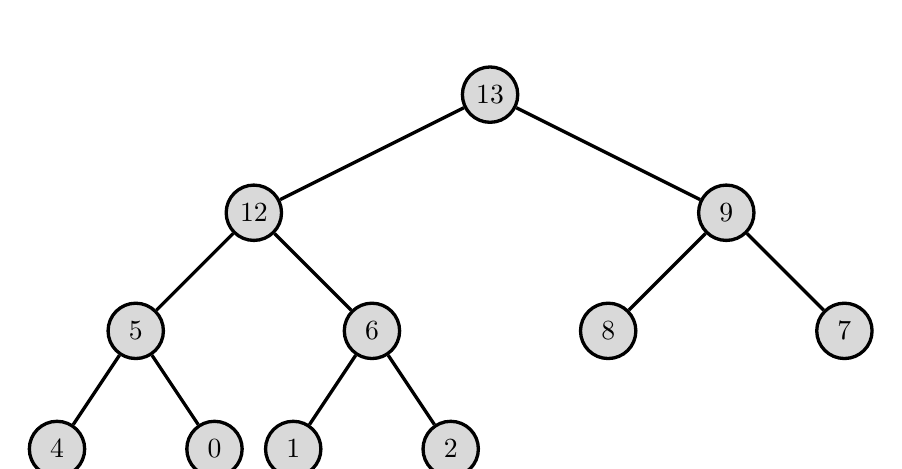
\begin{tikzpicture}[very thick,level/.style={sibling distance=60mm/#1}]
\node [vertex] {$13$}
  child {node [vertex] {$12$}
    child {node [vertex] {$5$}
      child {node [vertex] {$4$}}
      child {node [vertex] {$0$}}
    }
    child {node [vertex] {$6$}
      child {node [vertex] {$1$}}
      child {node [vertex] {$2$}}
    }
  }
  child {node [vertex] {$9$}
    child {node [vertex] {$8$}
    }
    child {node [vertex] {$7$}
    }
  };
\end{tikzpicture}
\caption*{Result of Max-Heapify. Return max = 15.}
\end{figure}
\newpage

\part{e}
Here follows an illustration of Max-Heap-Insert(A,11) on $A<15,13,9,5,12,8,7,4,0,6,2,1>$.\\
\vspace{5mm}
A.heapsize = A.heapsize + 1 = 12 + 1 = 13 \\
A[A.heapsize] = $-\infty \rightarrow$ A[13] = $-\infty$ \\
Heap-Increase-Key(A,A.heapsize,11) \\
A[A.heapsize] = key $\rightarrow$ A[13] = 11

\begin{figure}[htbp!]
\centering
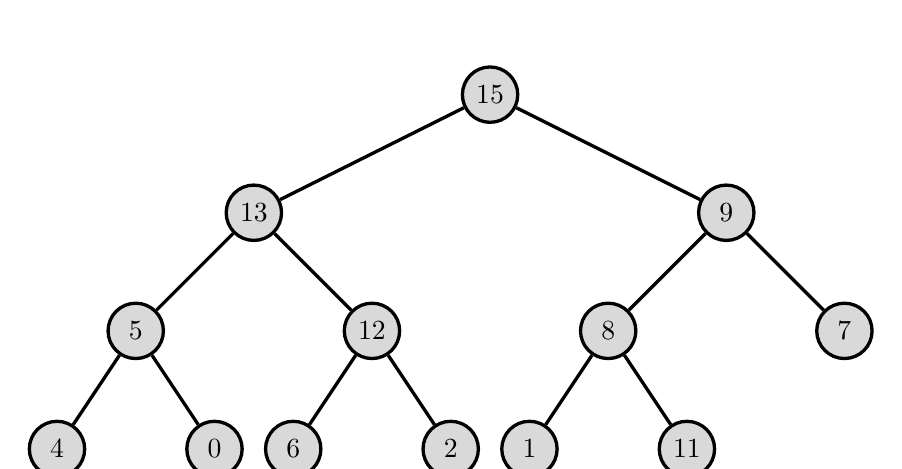
\begin{tikzpicture}[very thick,level/.style={sibling distance=60mm/#1}]
\node [vertex] {$15$}
  child {node [vertex] {$13$}
    child {node [vertex] {$5$}
      child {node [vertex] {$4$}}
      child {node [vertex] {$0$}}
    }
    child {node [vertex] {$12$}
      child {node [vertex] {$6$}}
      child {node [vertex] {$2$}}
    }
  }
  child {node [vertex] {$9$}
    child {node [vertex] {$8$}
      child {node [vertex] {$1$}}
      child {node [vertex] {$11$}}
    }
    child {node [vertex] {$7$}
    }
  };
\end{tikzpicture}
\caption*{}
\end{figure}

\begin{figure}[htbp!]
\centering
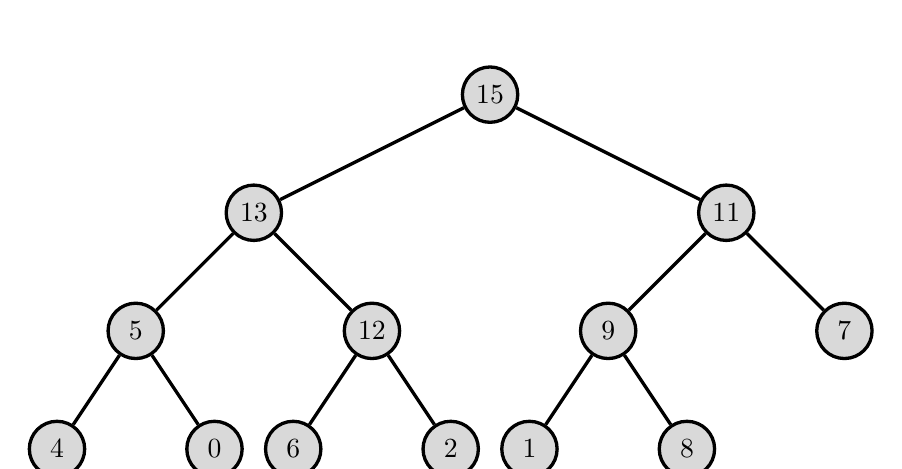
\begin{tikzpicture}[very thick,level/.style={sibling distance=60mm/#1}]
\node [vertex] {$15$}
  child {node [vertex] {$13$}
    child {node [vertex] {$5$}
      child {node [vertex] {$4$}}
      child {node [vertex] {$0$}}
    }
    child {node [vertex] {$12$}
      child {node [vertex] {$6$}}
      child {node [vertex] {$2$}}
    }
  }
  child {node [vertex] {$11$}
    child {node [vertex] {$9$}
      child {node [vertex] {$1$}}
      child {node [vertex] {$8$}}
    }
    child {node [vertex] {$7$}
    }
  };
\end{tikzpicture}
\caption*{The result of the while-loop of Heap-Increase-Key(A,A.heapsize,11).}
\end{figure}
\newpage

\question{Q2}{   Dutch Flag Problem}
This question can be solved using a partitioning method in manner similar to quicksort, utilizing three partitions and a swap() method. The partitions can be represented using three variables \textit{i, j,} and \textit{k}, setup initially as follows:

\begin{table}[htbp!]
\centering
\begin{tabular}{|l|l|l|l|l|l|}
\hline
i, j &  &  &  &  & k \\ \hline
\end{tabular}
\end{table}

Here follows Java/pseudocode for the partitioning:
\begin{lstlisting}
void DutchFlag(char[] A){
	int i = 0;
	int j = 0;
	int k = A.length-1;
	while (j <= k){
		// Case 1 - Put R character on left side at marker `i'
		if (A[j] == R){
			swap(A[i],A[j]);
			i++;
			j++
		}
		// Case 2 - Put W character in middle at marker `j'
		if (A[j] == W){
			j++
		}
		// Case 3 - Put B character on right side at marker `k'
		if (A[j] == B){
			swap(A[j],A[k]);
			k--;
		}
	}
}
\end{lstlisting}

This method ensures that all `R' characters are on the left side, all `B' characters are on the right side, and all `W' characters are in between by using \textit{i, j,} and \textit{k} as markers for where to insert/swap particular characters.

\question{Q3}{   CLRS 7-2}
\part{a}
From CLRS page 175, ``Worst case... partitioning routine produces one subproblem with n-1 elements and one with 0 elements.''

All elements being the same will produce this worst case event, as partition(A,p,r) returns r, so q=r and thus quicksort recursively calls quicksort(A,p,q-1) n-1 times. The recurrence relation for this is $T(n) = T(n-1) + \Theta(n)$ which evaluates to $\Theta(n^2)$ for this worst case when all elements are the same.

\part{b}
This can be done in a manner similar to Problem 2 (Dutch Flag Problem). The Java/pseudocode is as follows:

\begin{lstlisting}
PartitionPrime(A,p,r){
	int x = A[r];
	int j = p-1;
	int k = p-1;
	int t = r+1;
	for (int i = p; i <= r-1; i++){
		if (A[i] < x){
			j++;
			k++;
			swap(A[i],A[j]);
		}
		if (A[i] == x){
			k++;
			swap(A[i],A[k]);
		}
		if (A[i] > x){
			t--;
		}
	}
	swap(A[t-1],A[r]);
	return j,t;
}
\end{lstlisting}

This method utilizes a left partition $j$, a right partition $t$, and a middle partition $k$. It iterates through the array and places all elements equal to the partition value (A[r]) in the middle partition. Finally, it swaps partition value A[r] with the element at A[t-1] to complete the process.

\part{c}
\begin{lstlisting}
/*Java/Pseudocode for RandPartitionPrime*/
RandPartitionPrime(A,p,r){
	int i = Random(p,r);
	swap(A[r],A[i]);
	return PartitionPrime(A,p,r)
}
\end{lstlisting}

\begin{lstlisting}
/*Java/Pseudocode for RandQuicksortPrime*/
RandQuicksortPrime(A,p,r){
	if (p < r) {
		q,t = RandPartitionPrime(A,p,r);
		RandQuicksortPrime(A,p,q);
		RandQuicksortPrime(A,t,r);	
	}
}
\end{lstlisting}

\part{d}
Examine two cases:
\begin{enumerate}
	\item All elements distinct $\rightarrow$ O(n lg n).
	\item All elements identical $\rightarrow$ O(n).
\end{enumerate}
Number (2) is true because O(n) work is performed at each level but the recursion tree depth is simply 1, not lg n, because we do not recurse on elements equal to the initial pivot (which is all of them).

Thus, the time complexity of this modified Quicksort, QuicksortPrime, is O(n lg n) and the worst case occurs when there no duplicate elements.

\question{Q4}{}
\part{a}
The following table demonstrates Radix Sort.
\begin{figure}[htbp!]
  \centering
  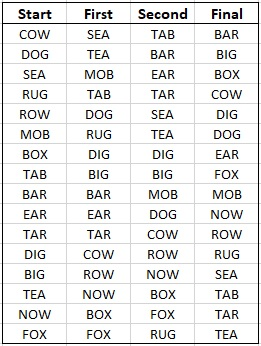
\includegraphics{one.jpg}
\end{figure}

\part{b}
The following table demonstrates Bucket Sort.
\begin{figure}[htbp!]
  \centering
  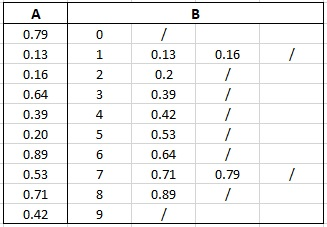
\includegraphics{two.jpg}
\end{figure}
\newpage

\part{c}
Bucket Sort assumes a uniform distribution. The reason why Bucket Sort is $\Theta(n^2)$ is perhaps best illustrated with an example. Consider two cases.
\begin{enumerate}
	\item Ten elements in ten buckets with insertion sort $O(n^2)$ yields $10(1^2) = 10$.
	\item Ten elements in one bucket with insertion sort $O(n^2)$ yields $1(10^2) = 100$.
\end{enumerate}
Clearly, the worst case is $O(n^2)$. If we simply use a sort more efficient than Insertion Sort (such as Merge Sort), then performance can be improved to O(n lg n).

\question{Q5}{}
\part{a}
First, compare pairs of elements to find the lowest. Compare ``winners'' in pairs to find the lowest. Repeat until only one remains (the minimum value).

To find the second lowest, compare the lg n ``losers''. This gives (n-1) comparisons to find the minimum and (lg n - 1) comparisons to find the second minimum.

See the following example.

\begin{figure}[htbp!]
\centering
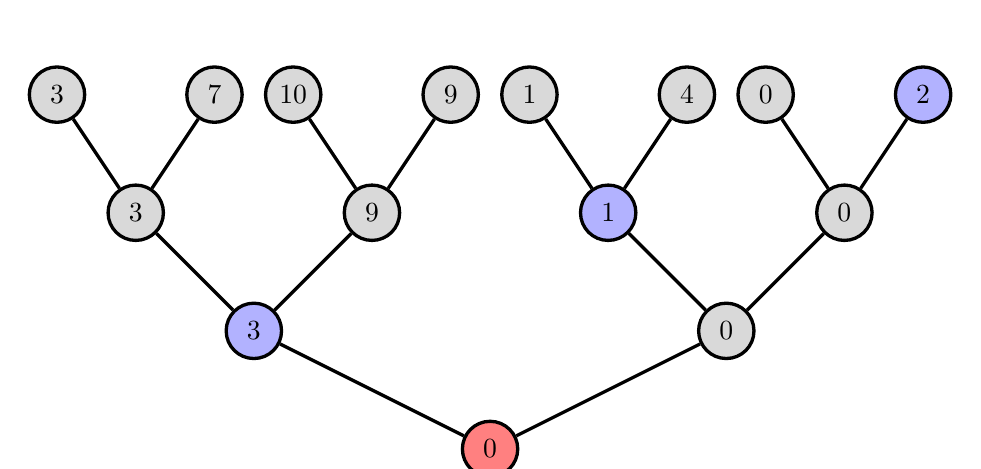
\begin{tikzpicture}[grow'=up,very thick,level/.style={sibling distance=60mm/#1}]
\node [vertex, fill=red!50] {$0$}
  child {node [vertex, fill=blue!30] {$3$}
    child {node [vertex] {$3$}
      child {node [vertex] {$3$}}
      child {node [vertex] {$7$}}
    }
    child {node [vertex] {$9$}
      child {node [vertex] {$10$}}
      child {node [vertex] {$9$}}
    }
  }
  child {node [vertex] {$0$}
    child {node [vertex, fill=blue!30] {$1$}
      child {node [vertex] {$1$}}
      child {node [vertex] {$4$}}
    }
    child {node [vertex] {$0$}
      child {node [vertex] {$0$}}
      child {node [vertex, fill=blue!30] {$2$}}
    }
  };
\end{tikzpicture}
\caption*{The main bracket to find the lowest. Note that n - 1 comparisons are made.}
\end{figure}

\begin{figure}[htbp!]
\centering
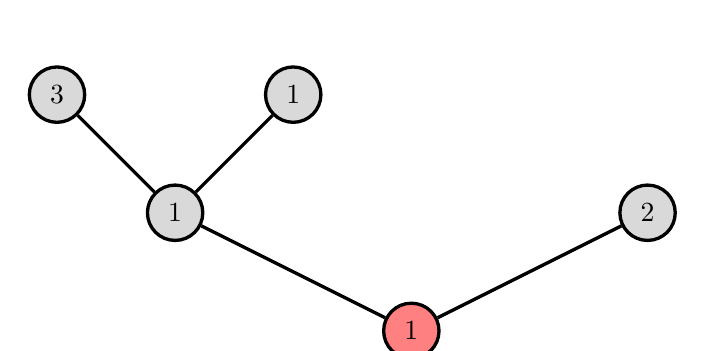
\begin{tikzpicture}[grow'=up,very thick,level/.style={sibling distance=60mm/#1}]
\node [vertex, fill=red!50] {$1$}
  child {node [vertex] {$1$}
    child {node [vertex] {$3$}
    }
    child {node [vertex] {$1$}
    }
  }
  child {node [vertex] {$2$}
  };
\end{tikzpicture}
\caption*{The ``loser'' bracket to find the second lowest. Note that lg n - 1 comparisons are made.}
\end{figure}
\newpage
From this, we can see that the two smallest elements were found with only $n + \ceil{lg n} - 2$ comparisons.

\part{b}
It is helpful to construct a diagram for this problem. In the figure below, we examine several possible locations for and east-west pipeline. However, only one choice provides the minimum distance for secondary pipelines. The ideal location then of the primary east-west pipline is located at the north-south axis (y-axis) median of the oil wells. To achieve this in linear time, we can simply use the Select() algorithm to determine the value of the median by finding the (n/2)\textsuperscript{th} smallest element (when n is odd) and the average of the $\ceil{(n+1)/2}$\textsuperscript{th} and $\floor{(n+1)/2}$\textsuperscript{th} smallest elements (when n is even).
\begin{figure}[htbp!]
  \centering
  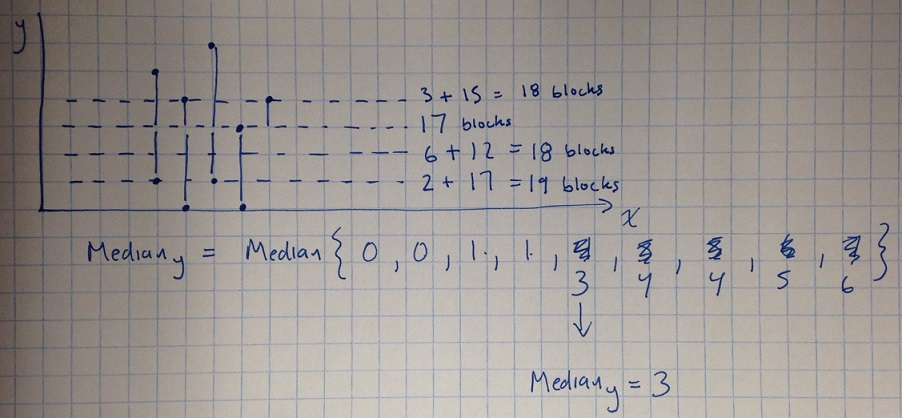
\includegraphics[width=\textwidth]{IMG_0401.jpg}
\end{figure}

\question{Q6}{   CLRS 14.1-5}
This can be done via the follow method:
\begin{lstlisting}
/*Java/pseudocode for Successor method*/
Successor(T,x,i){
	rank = OS-RANK(T,x);
	pos = rank+i;
	successor = OS-SELECT(T.root,pos);
	return successor;
}	
\end{lstlisting}


\end{document}









